% +--------------------------------------------------------------------+
% | Appendix A Page (Optional)                                         |
% +--------------------------------------------------------------------+

\cleardoublepage

\chapter{\projectName{} Use-Case Screenshots}
\label{Appendix:Key1}

\begin{figure}[htb]%t=top, b=bottom, h=here

    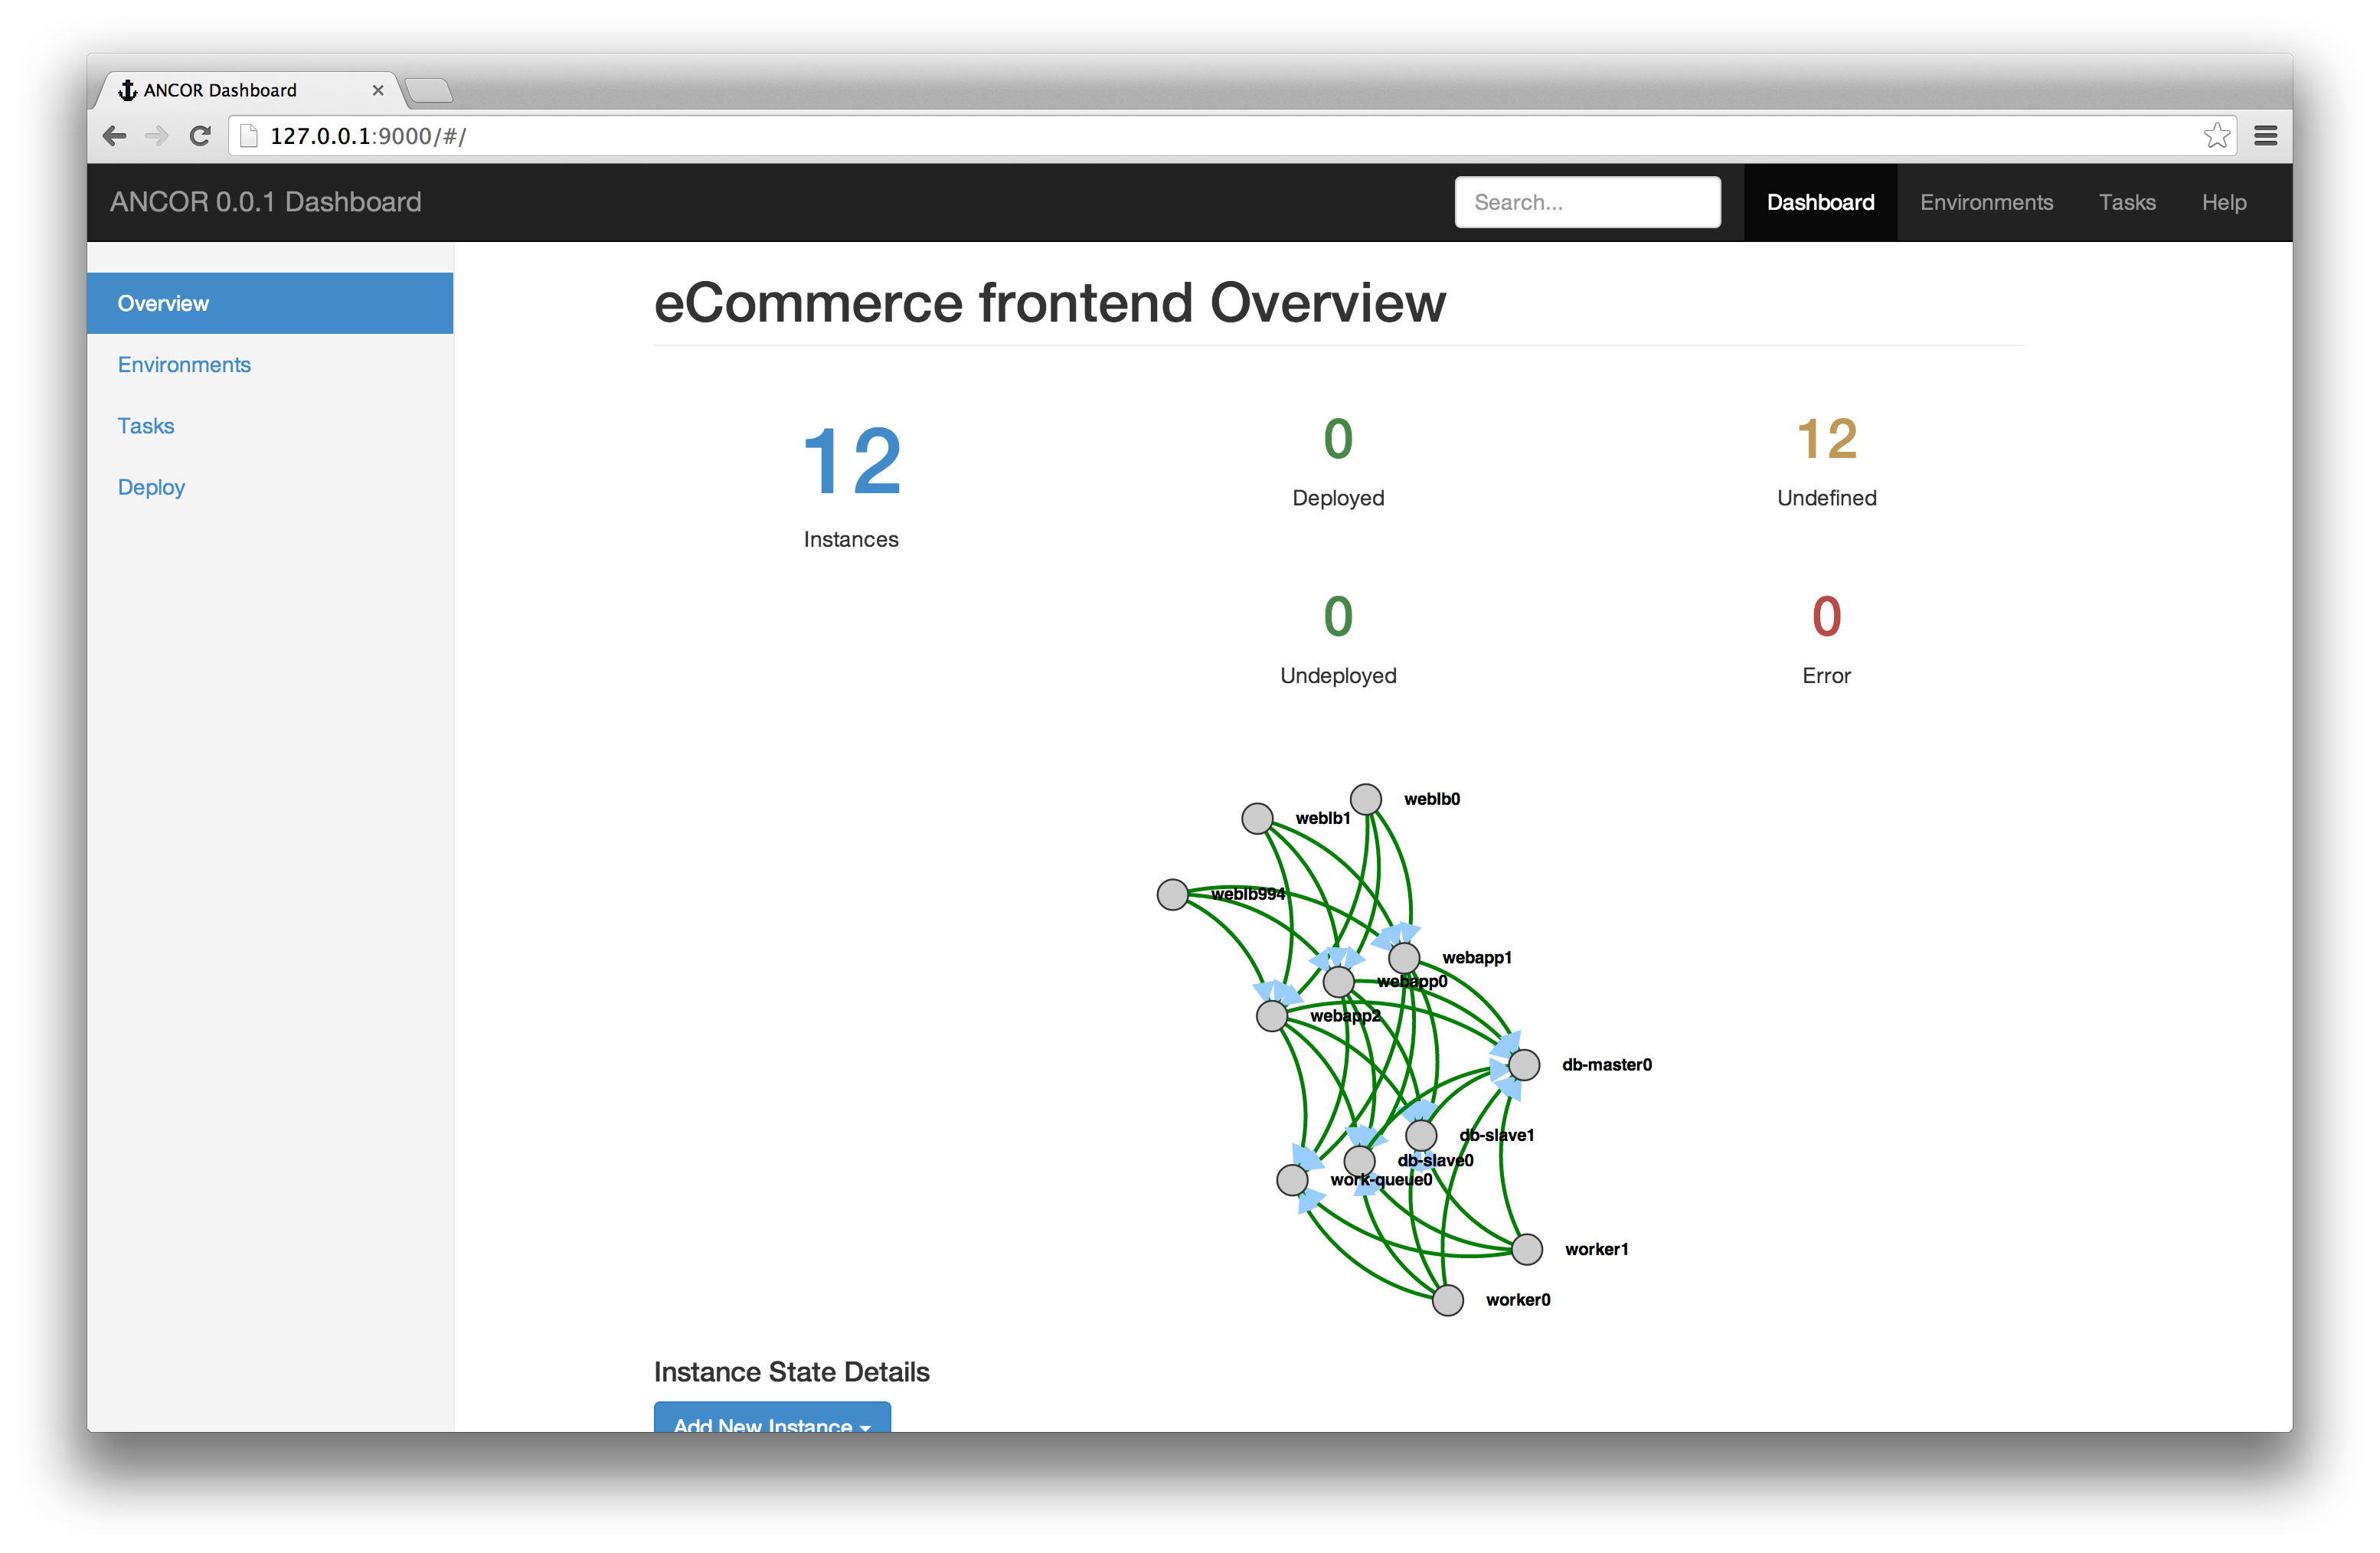
\includegraphics[height=4.0in]{figures/viewing-instances-main.png}

    \caption[The main view of a deployed ANCOR system.
    ]{The main view of a deployed ANCOR system.}

    \label{mainInstanceView}
\end{figure}

\begin{figure}[htb]%t=top, b=bottom, h=here

    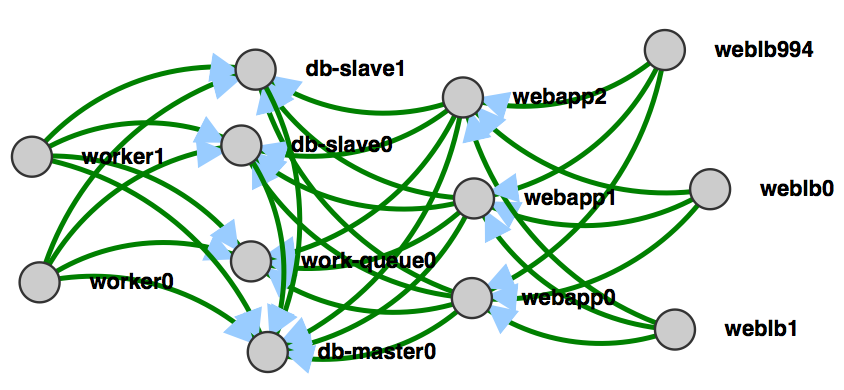
\includegraphics[height=3.0in]{figures/network-graph.png}

    \caption[D3.js Network Graph
    ]{A dynamically generated network graph.}

    \label{networkGraph}
\end{figure}

\begin{figure}[htb]%t=top, b=bottom, h=here

    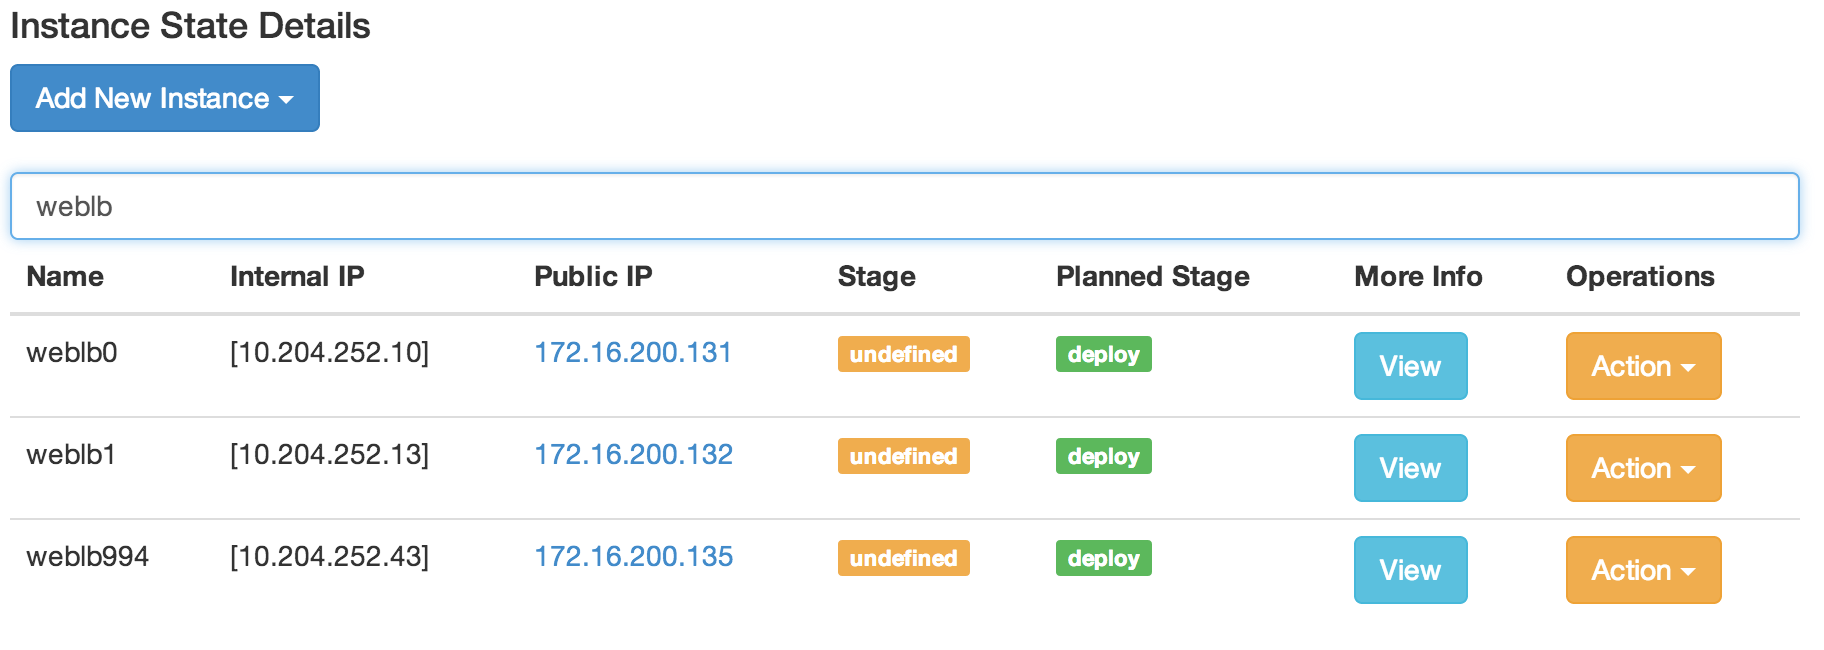
\includegraphics[height=2.3in]{figures/instance-table-filter.png}

    \caption[A user searching for weblb from the instance table.
    ]{A user searching for weblb from the instance table.}

    \label{instanceTableFilter}
\end{figure}

\begin{figure}[htb]%t=top, b=bottom, h=here

    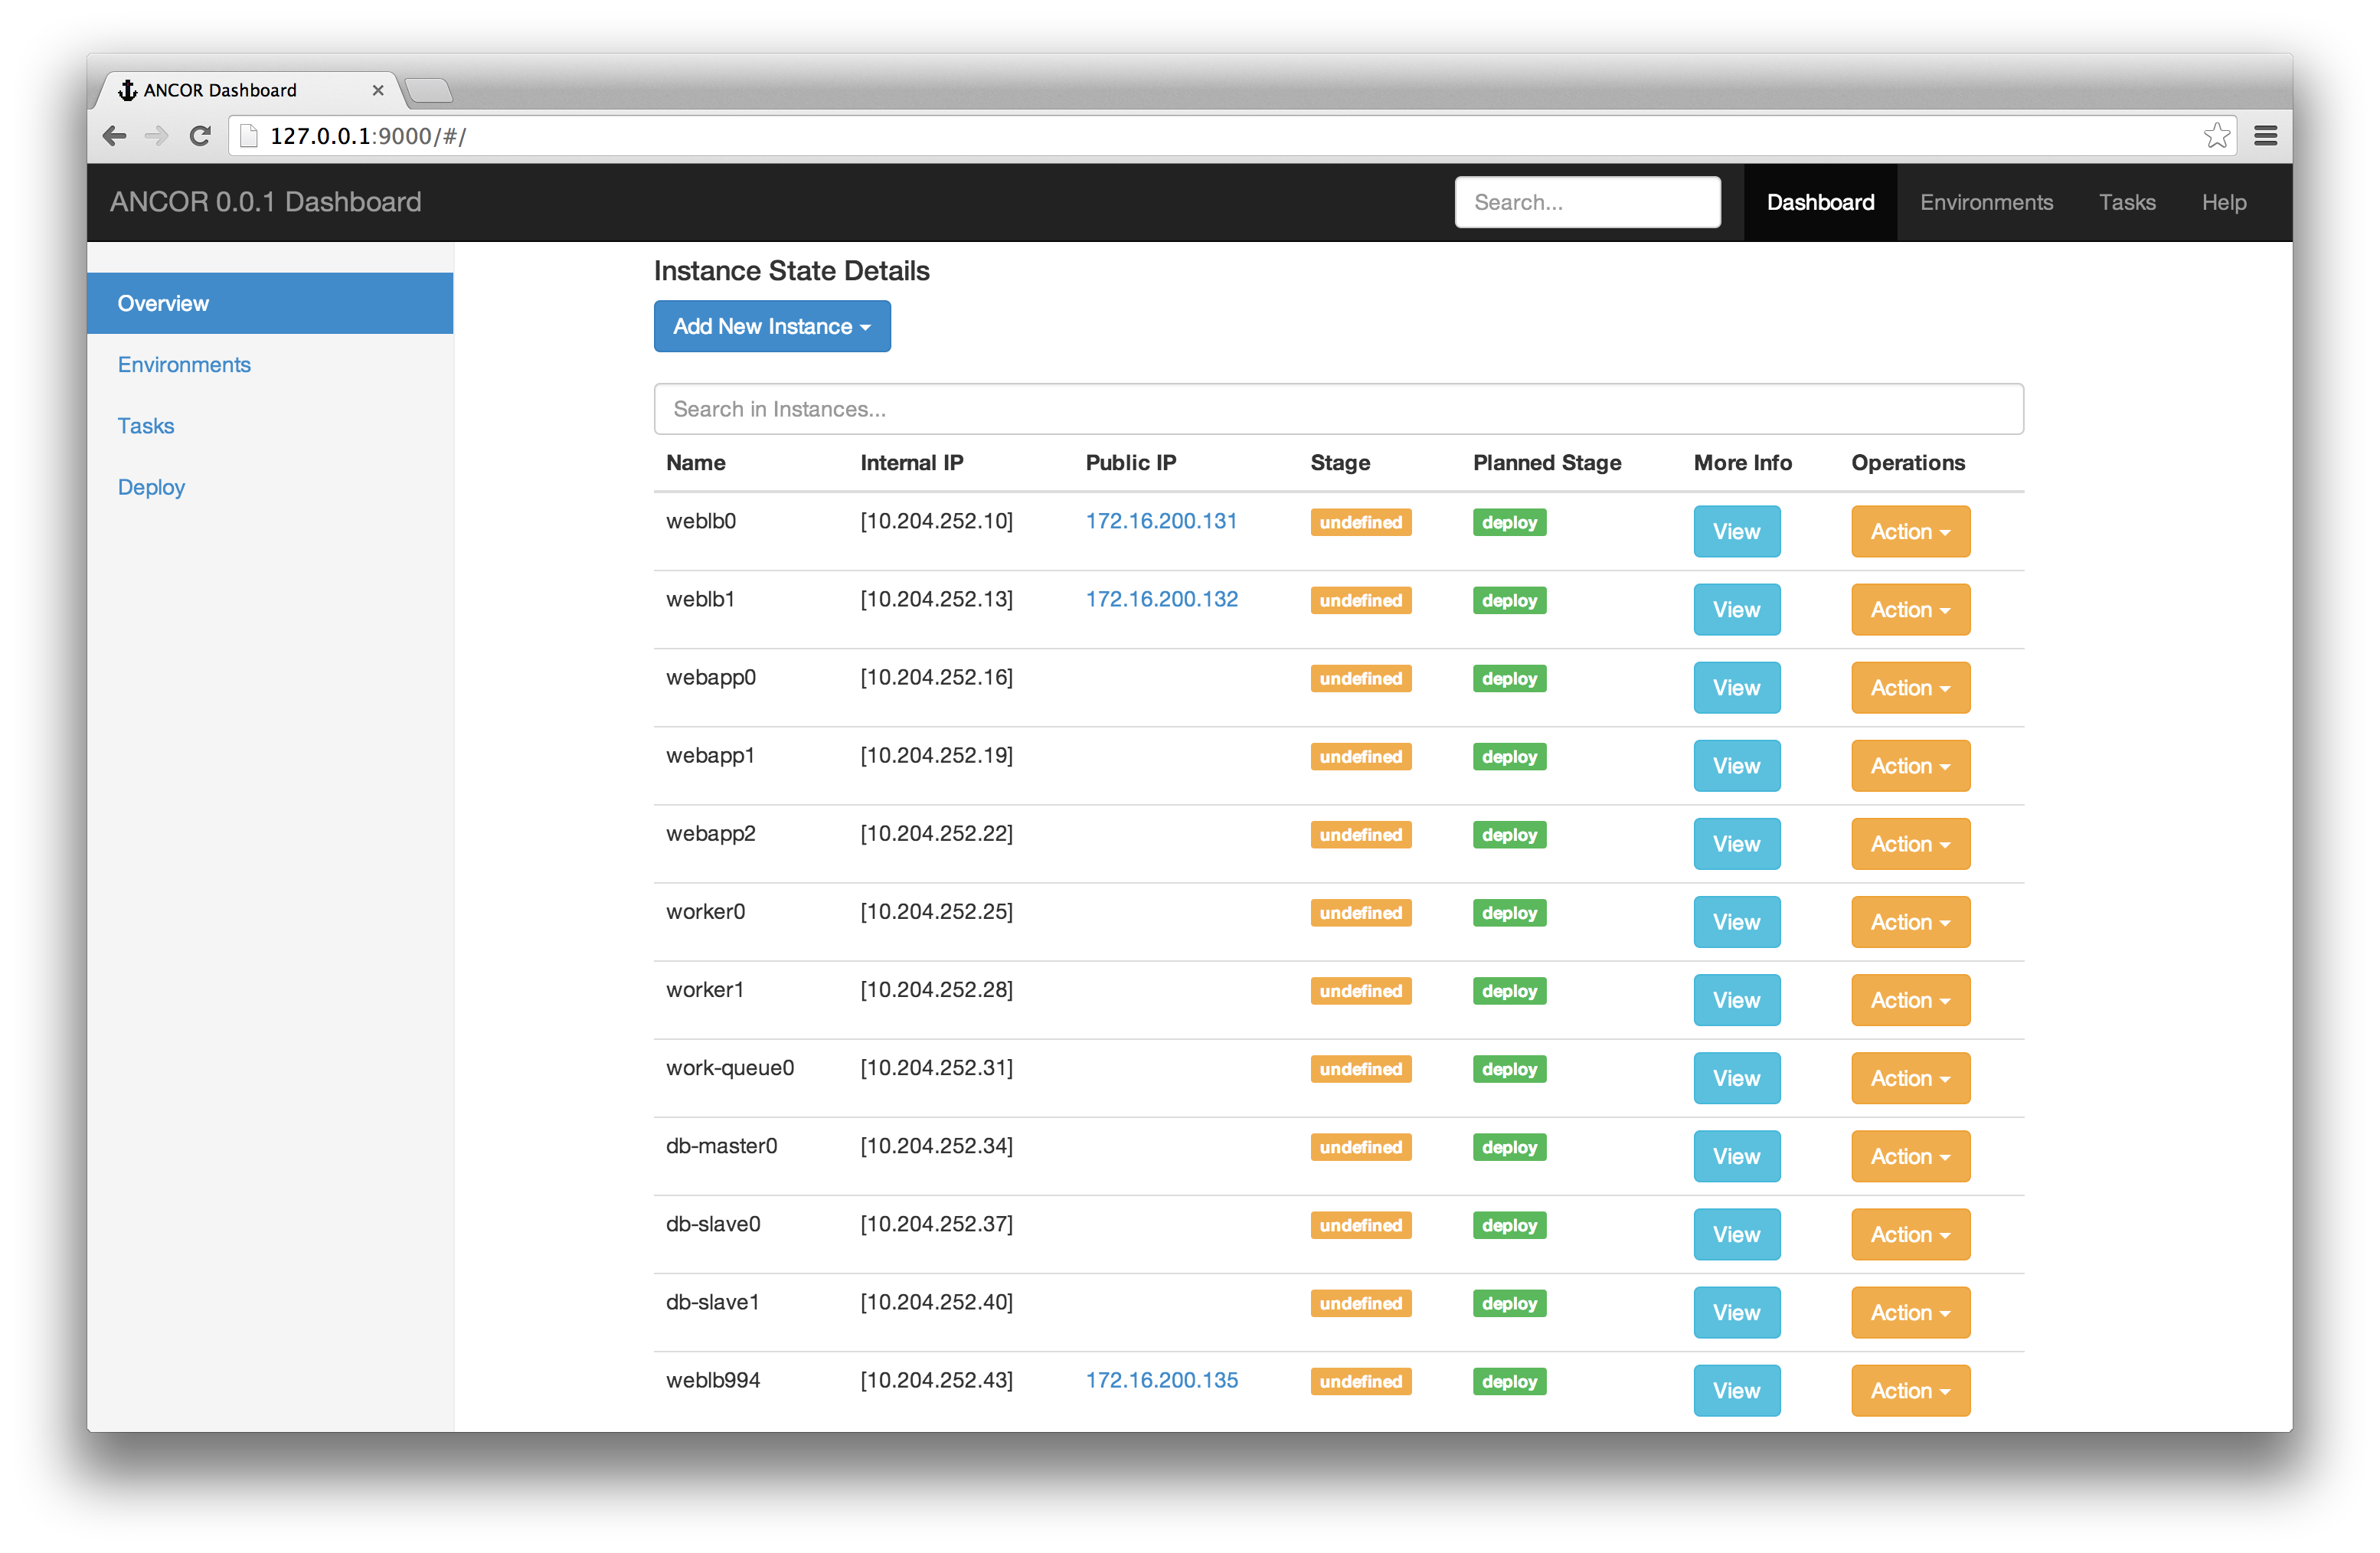
\includegraphics[height=4.0in]{figures/instance-table-view.png}

    \caption[Instance table view.
    ]{The instance table shown on the main view.}

    \label{mainInstanceTableView}
\end{figure}

\begin{figure}[htb]%t=top, b=bottom, h=here

    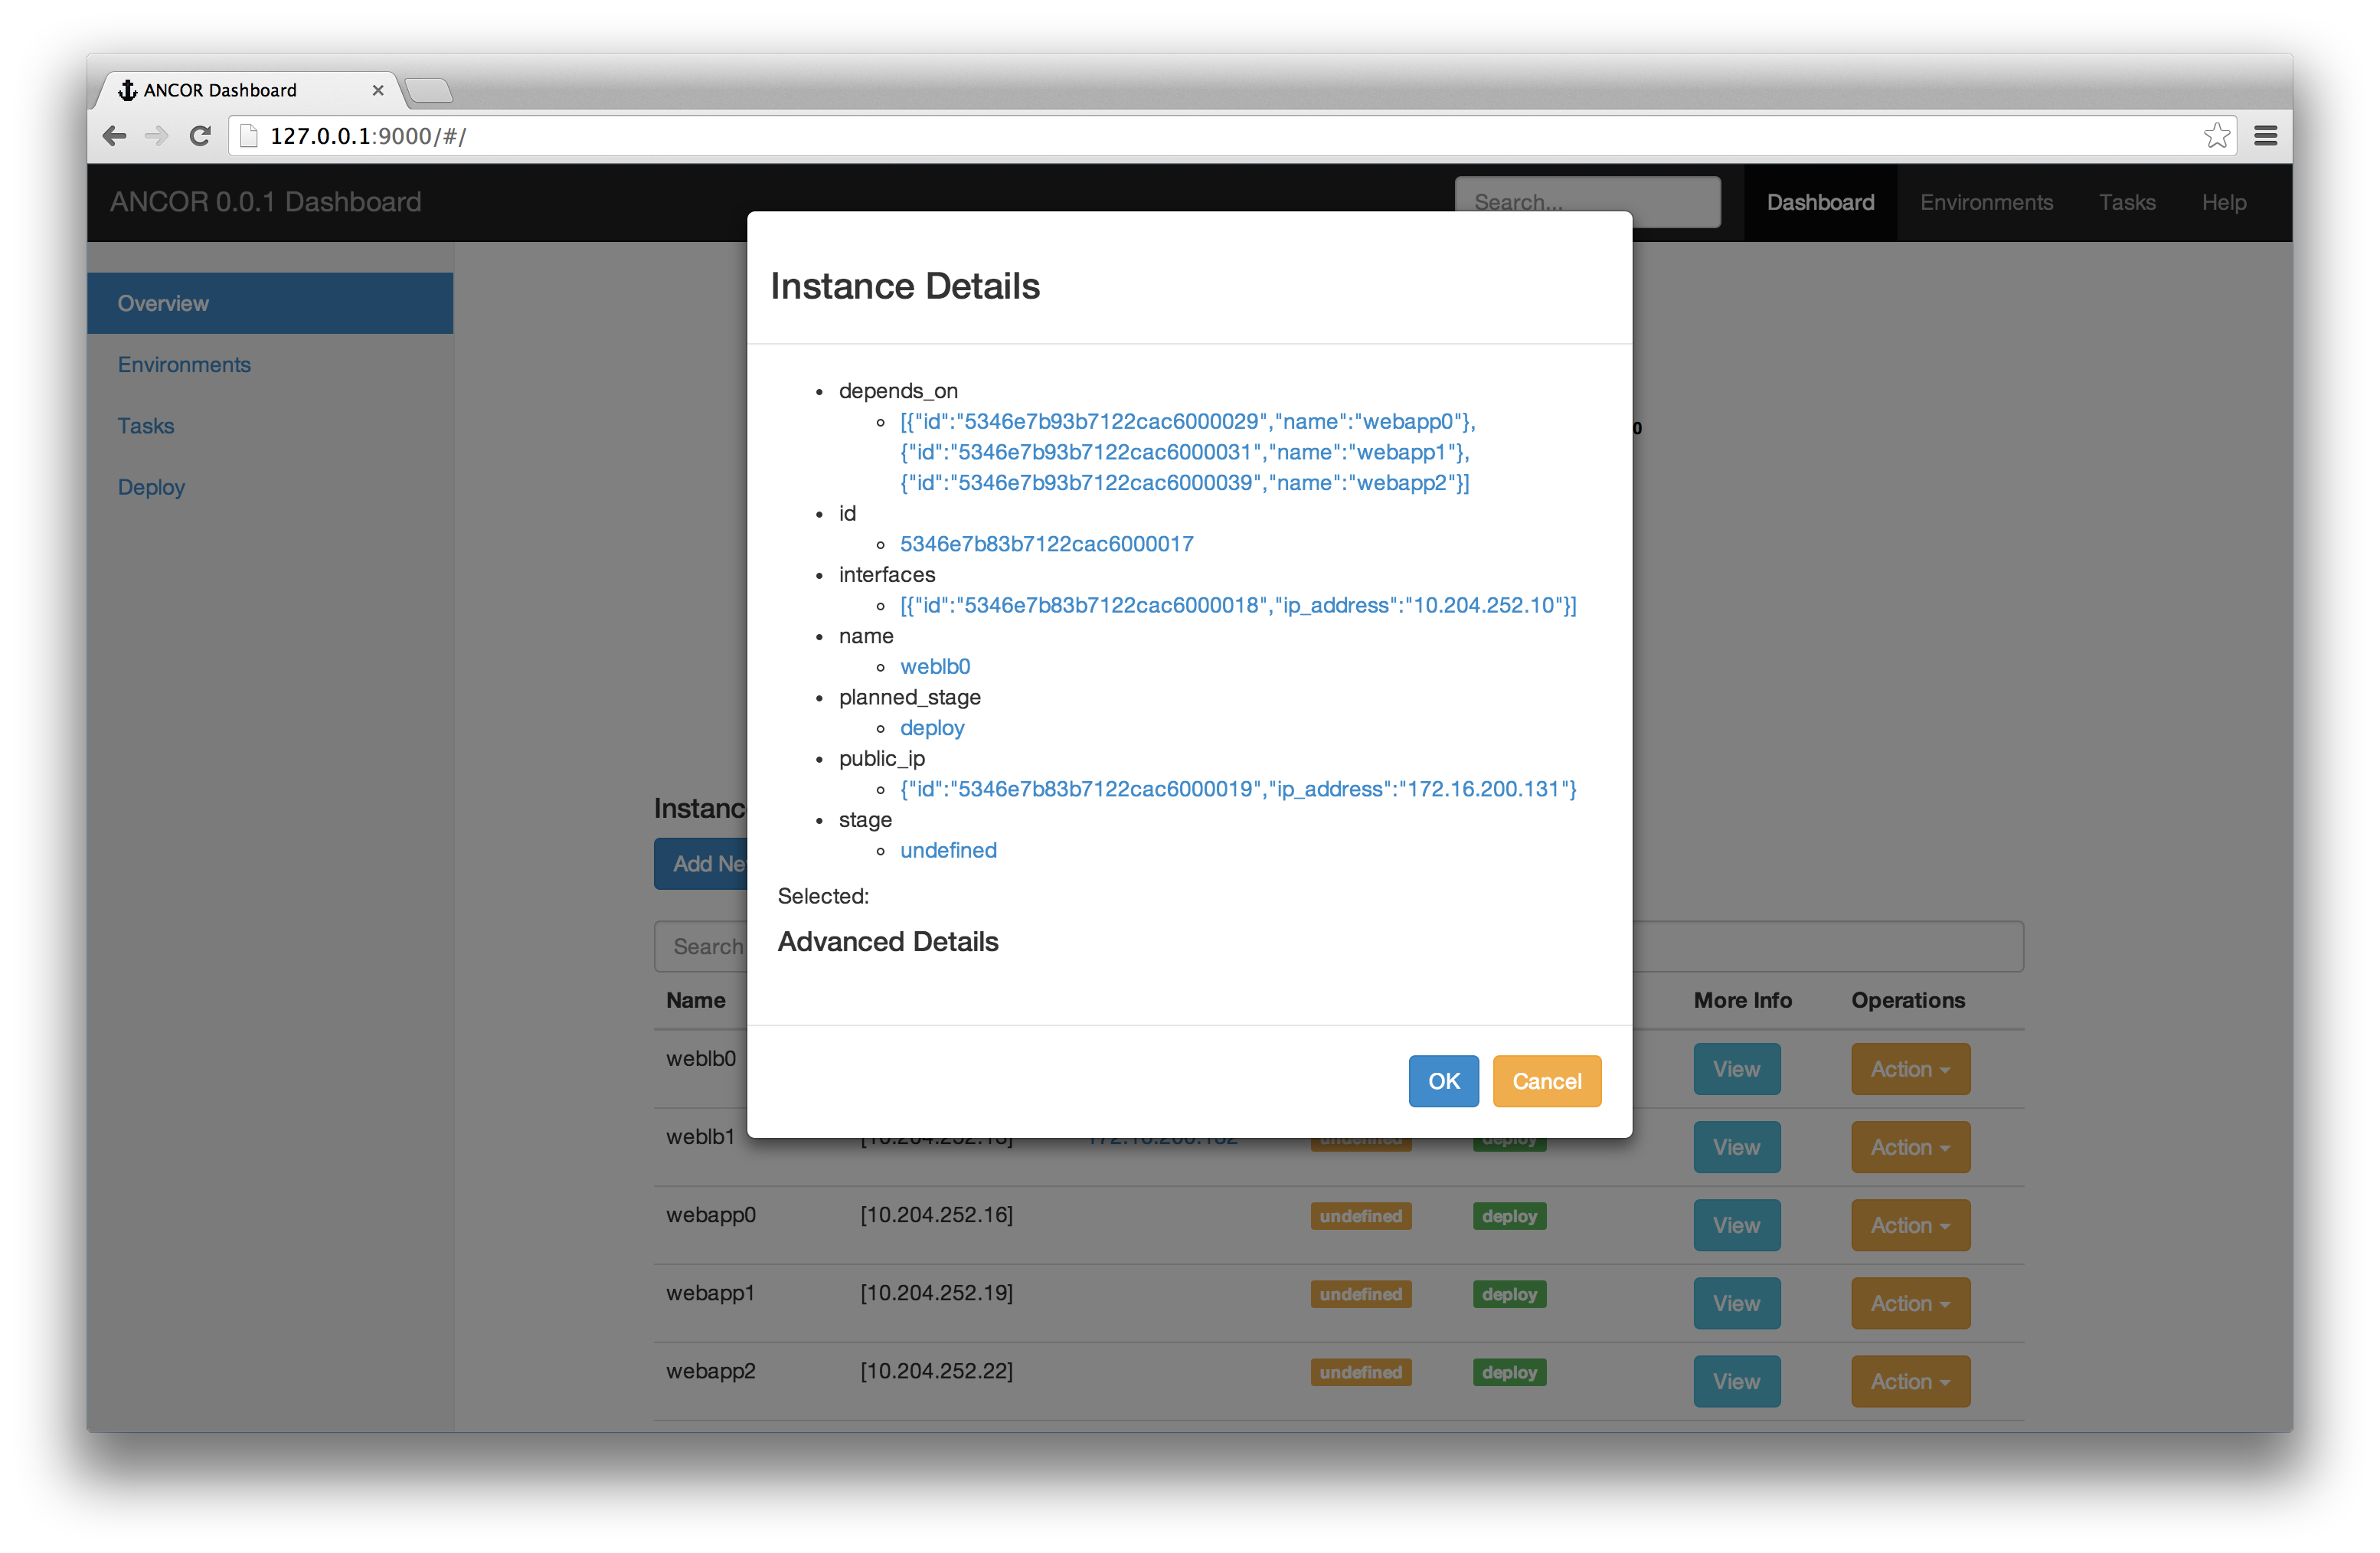
\includegraphics[height=4.0in]{figures/instance-modal-view.png}

    \caption[Instance modal view.
    ]{The instance modal view shown when a user wants more information.}

    \label{modalInstanceView}
\end{figure}

\begin{figure}[htb]%t=top, b=bottom, h=here

    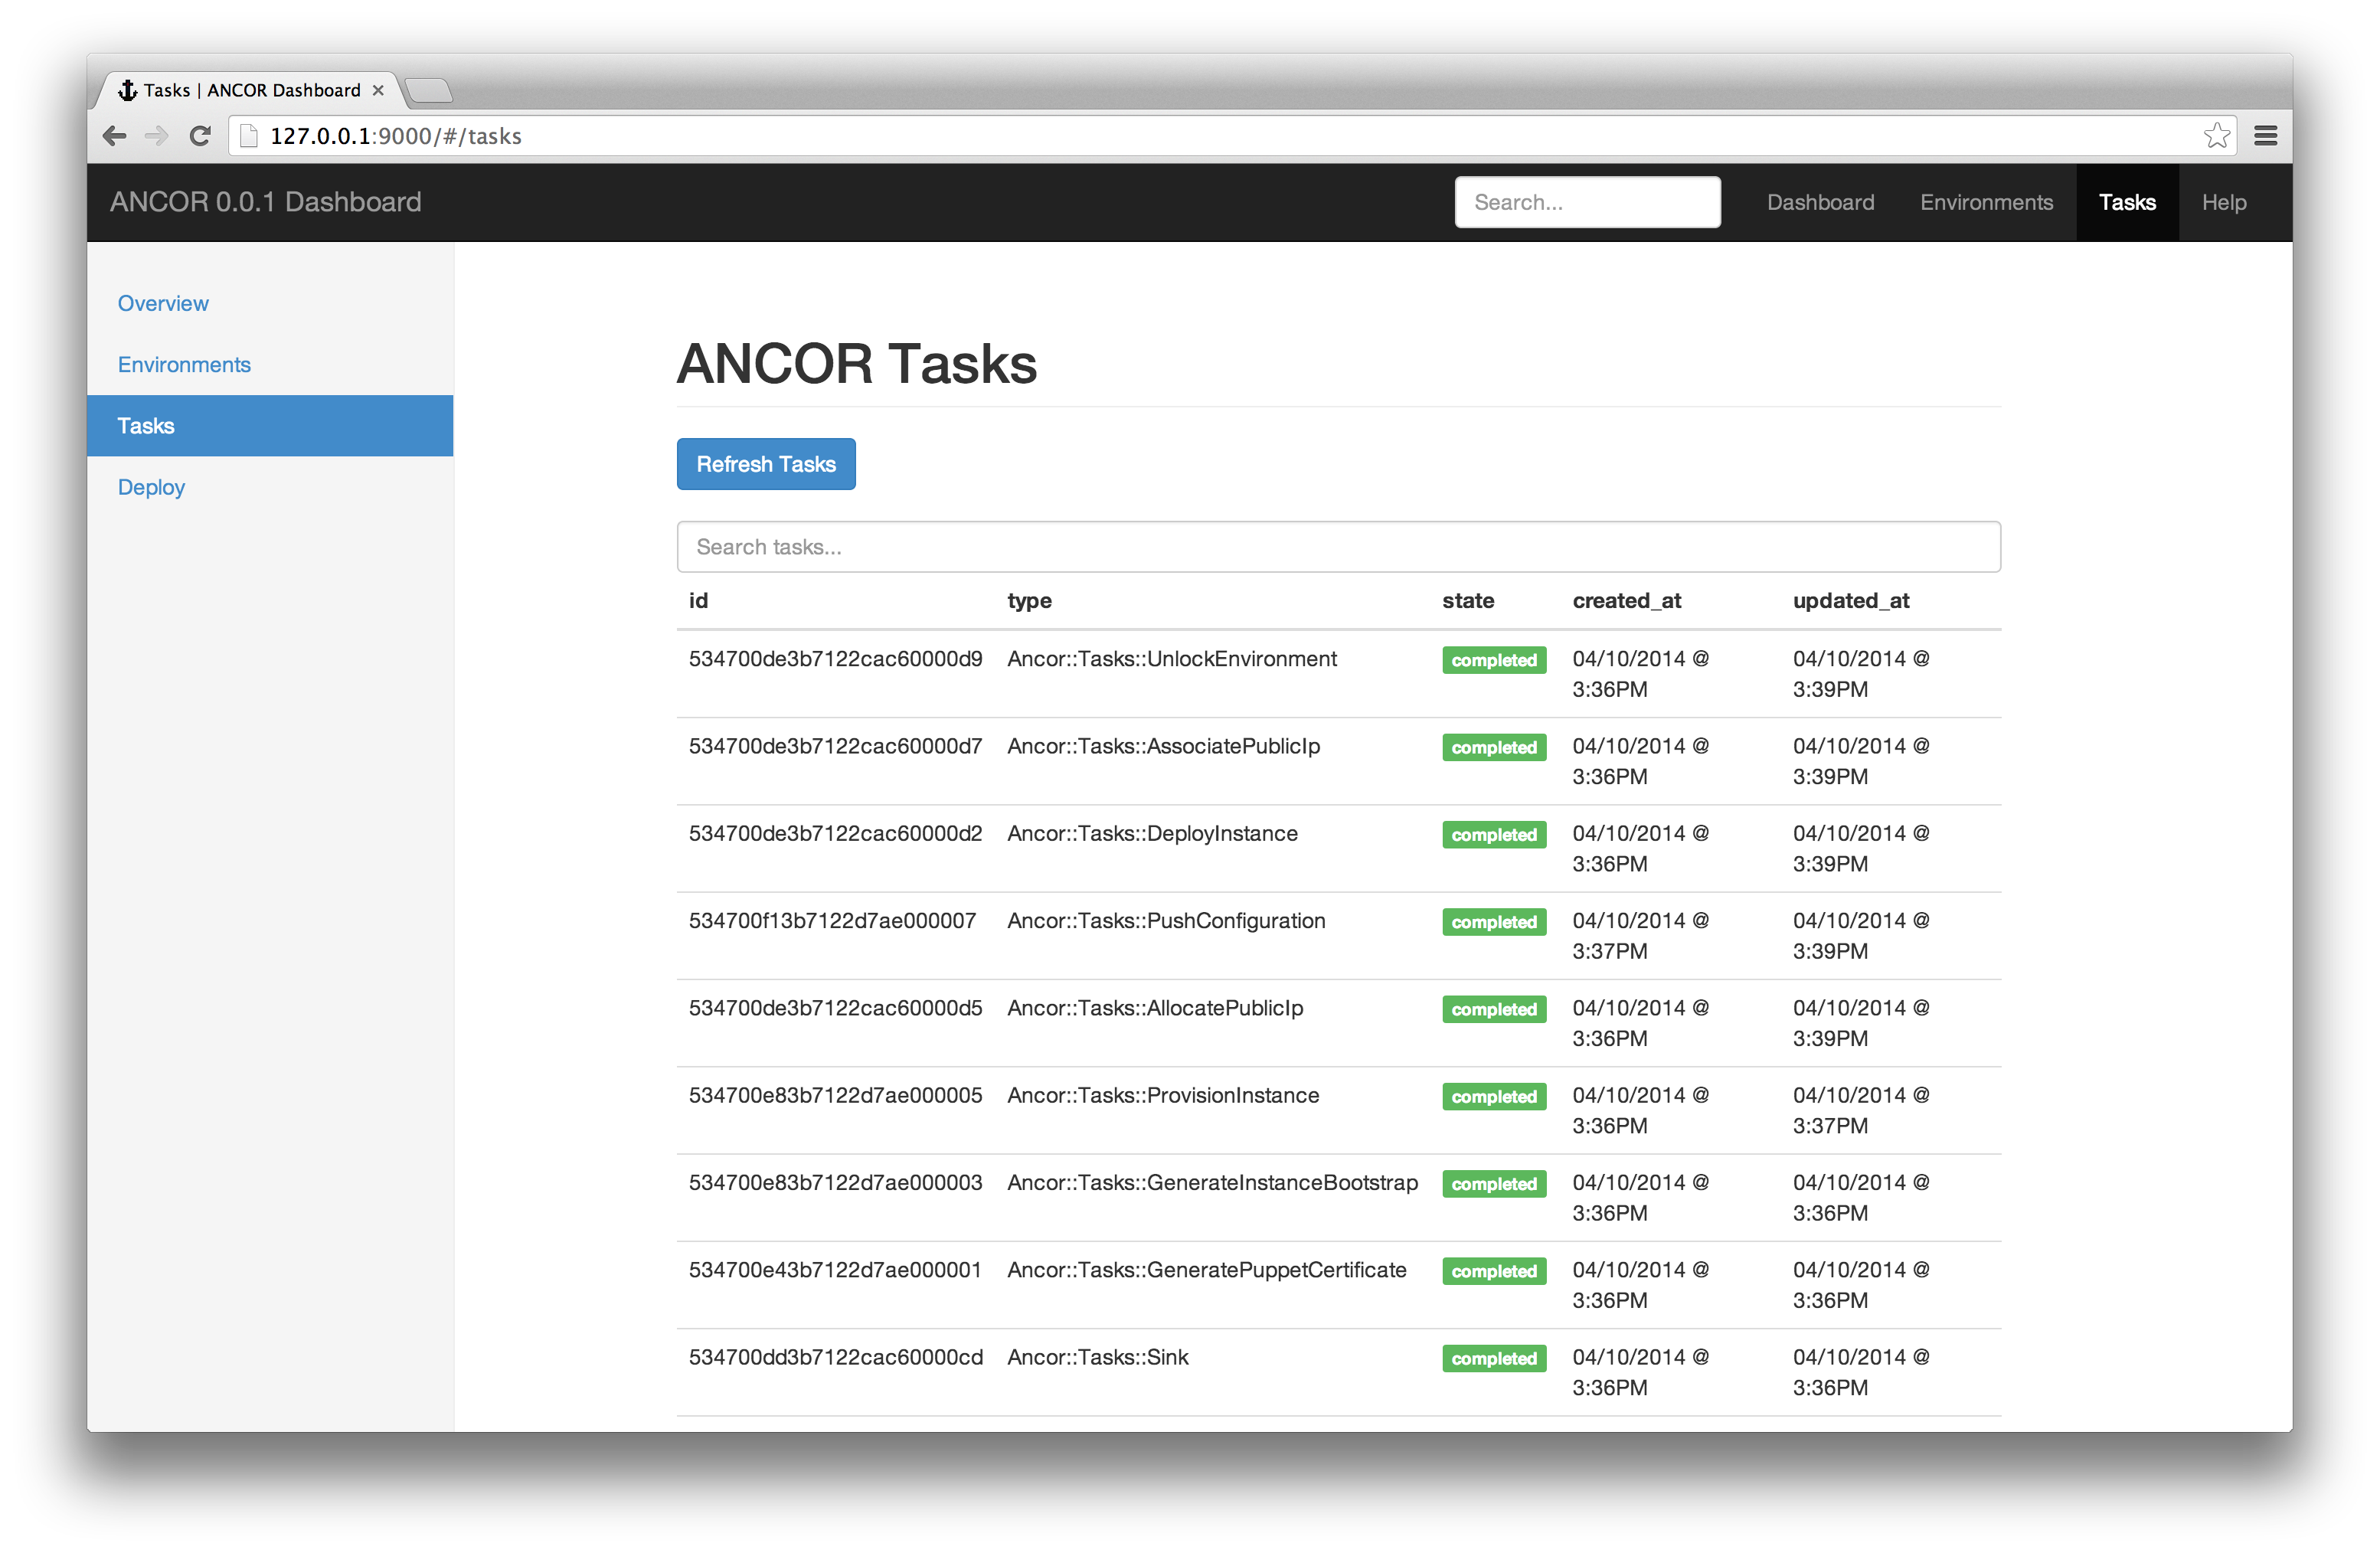
\includegraphics[height=4.0in]{figures/tasks.png}

    \caption[Tasks view.
    ]{A list of all current Tasks.}

    \label{tasksView}
\end{figure}

\begin{figure}[htb]%t=top, b=bottom, h=here

    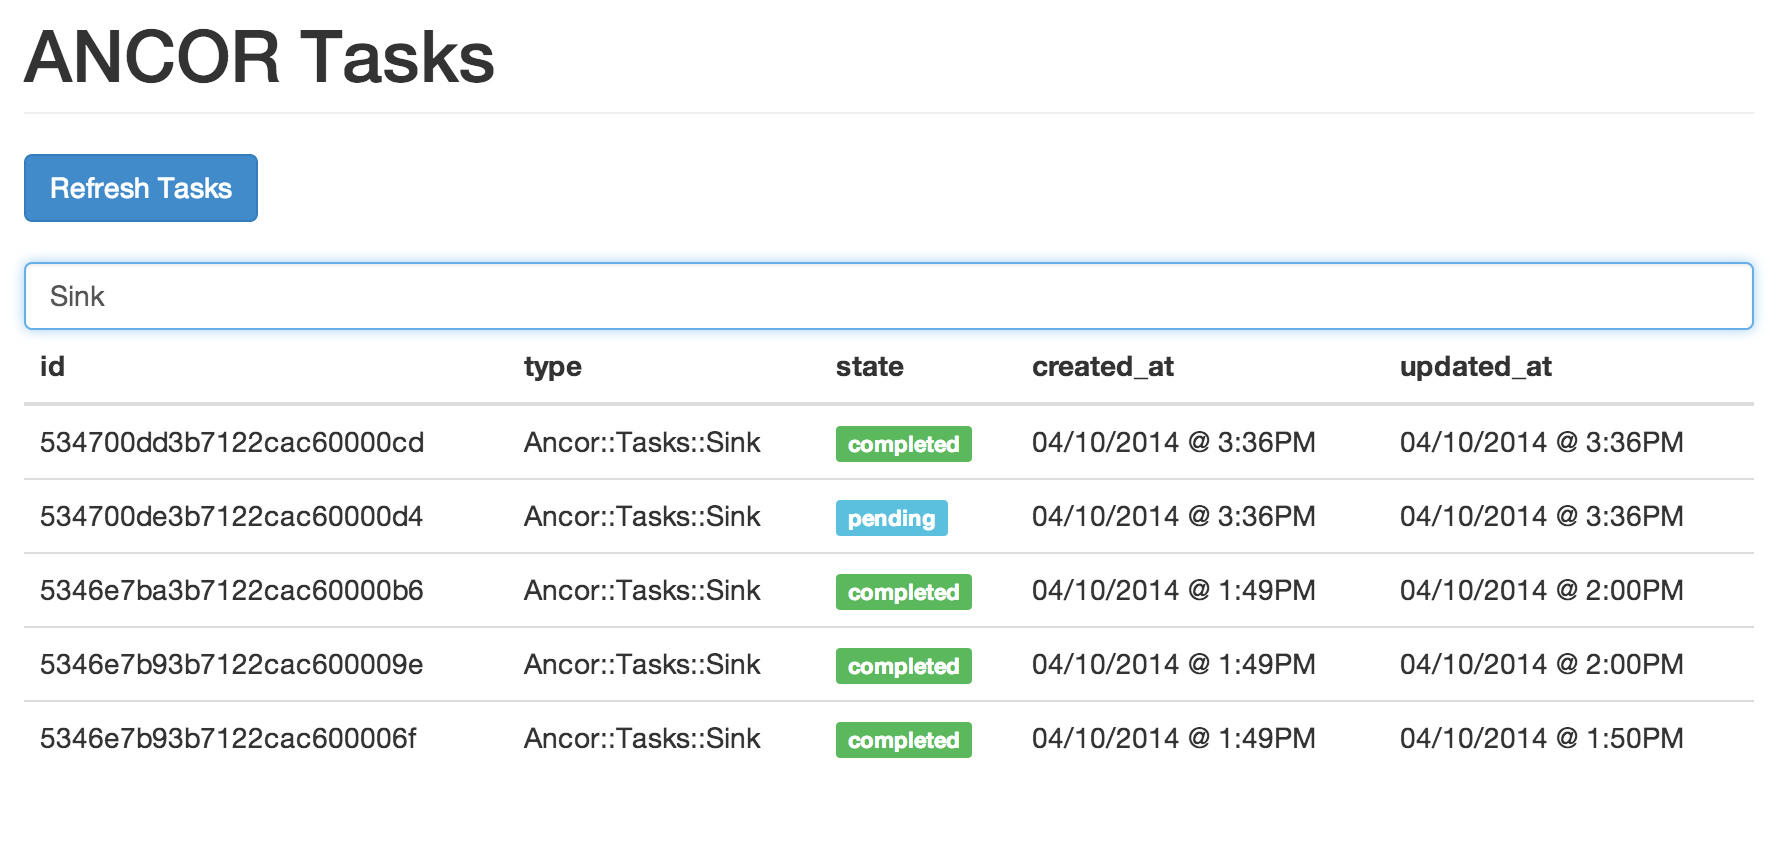
\includegraphics[height=3.0in]{figures/tasks-filter.png}

    \caption[Tasks filter view.
    ]{A filtered list of all current Tasks related to Sink.}

    \label{tasksFilter}
\end{figure}

\begin{figure}[htb]%t=top, b=bottom, h=here

    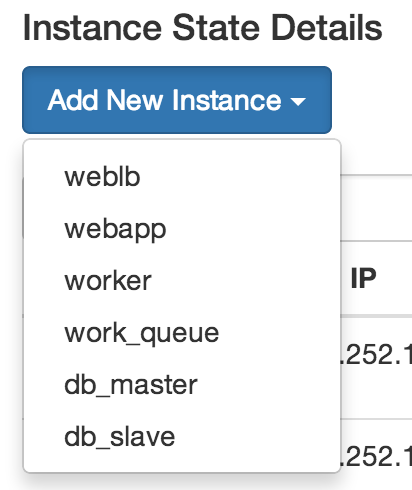
\includegraphics[height=3.0in]{figures/instance-dropdown.png}

    \caption[A dropdown of all current instances/roles.
    ]{A dropdown of all the current instances/roles to add to the deployment.}

    \label{dropdownRoles}
\end{figure}

\begin{figure}[htb]%t=top, b=bottom, h=here

    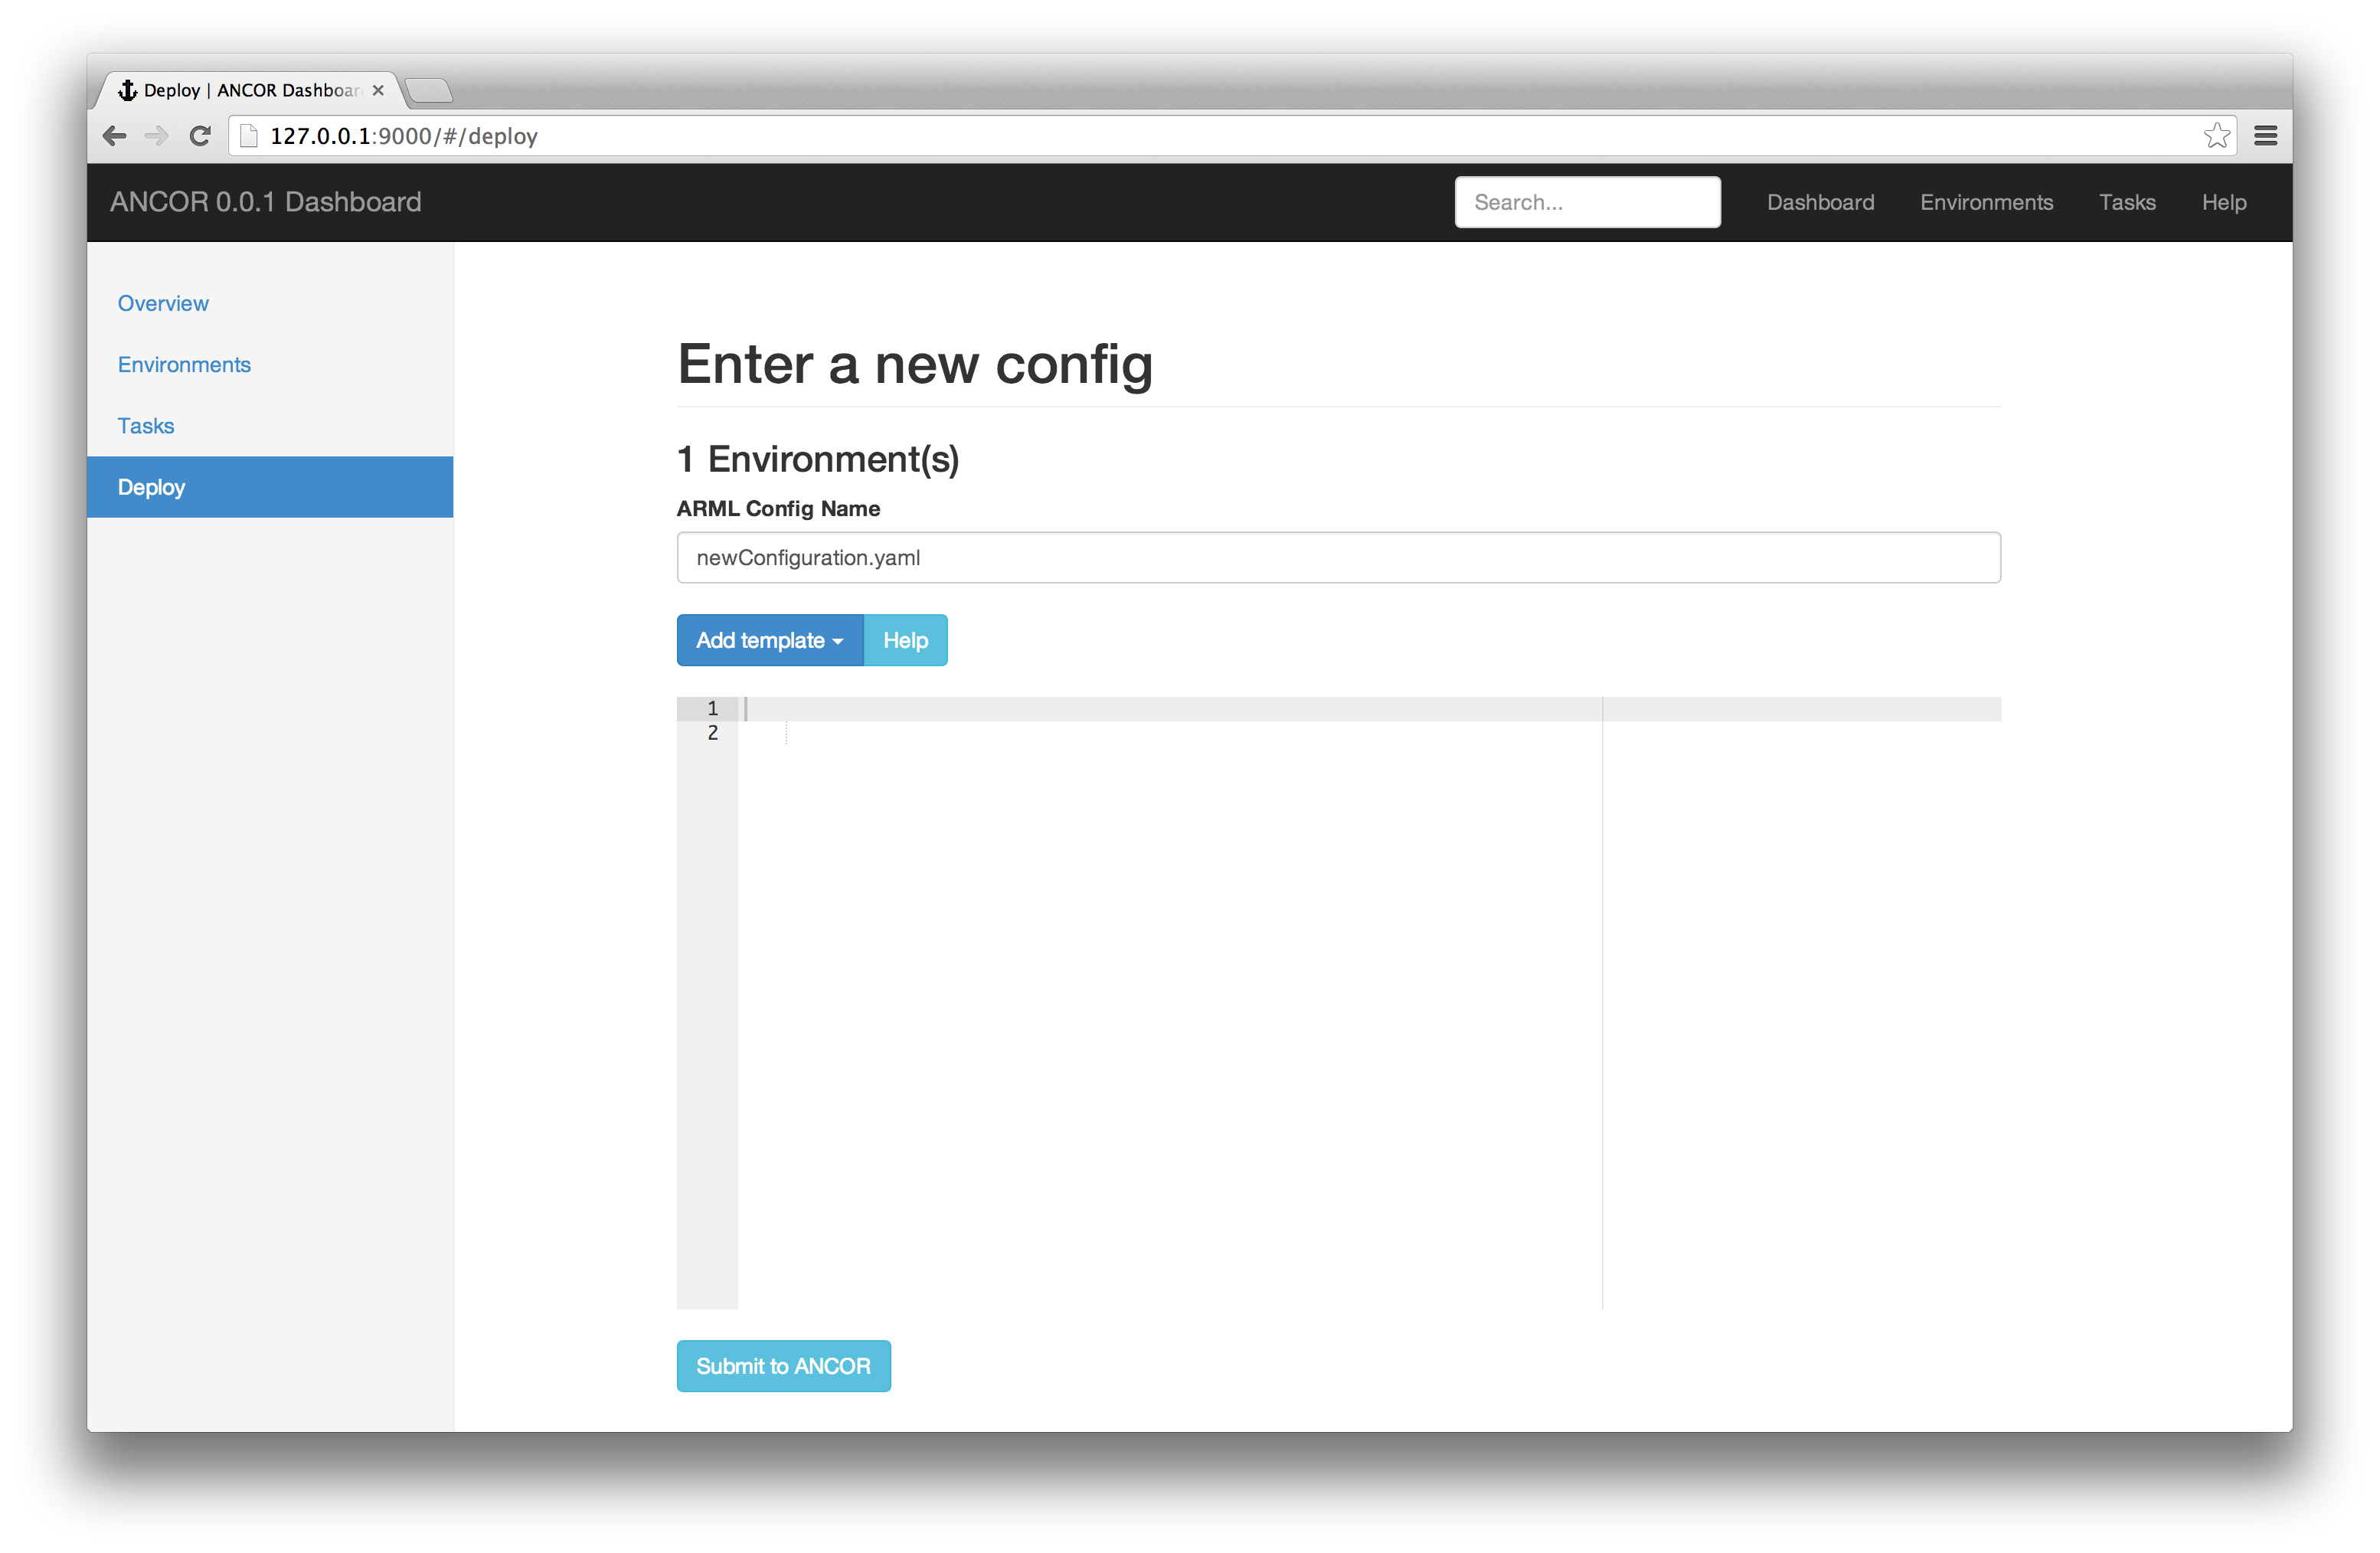
\includegraphics[height=4.0in]{figures/deploy.png}

    \caption[Deploy view.
    ]{The deploy view, where users can write their own configuration file.}

    \label{deployView}
\end{figure}

\begin{figure}[htb]%t=top, b=bottom, h=here

    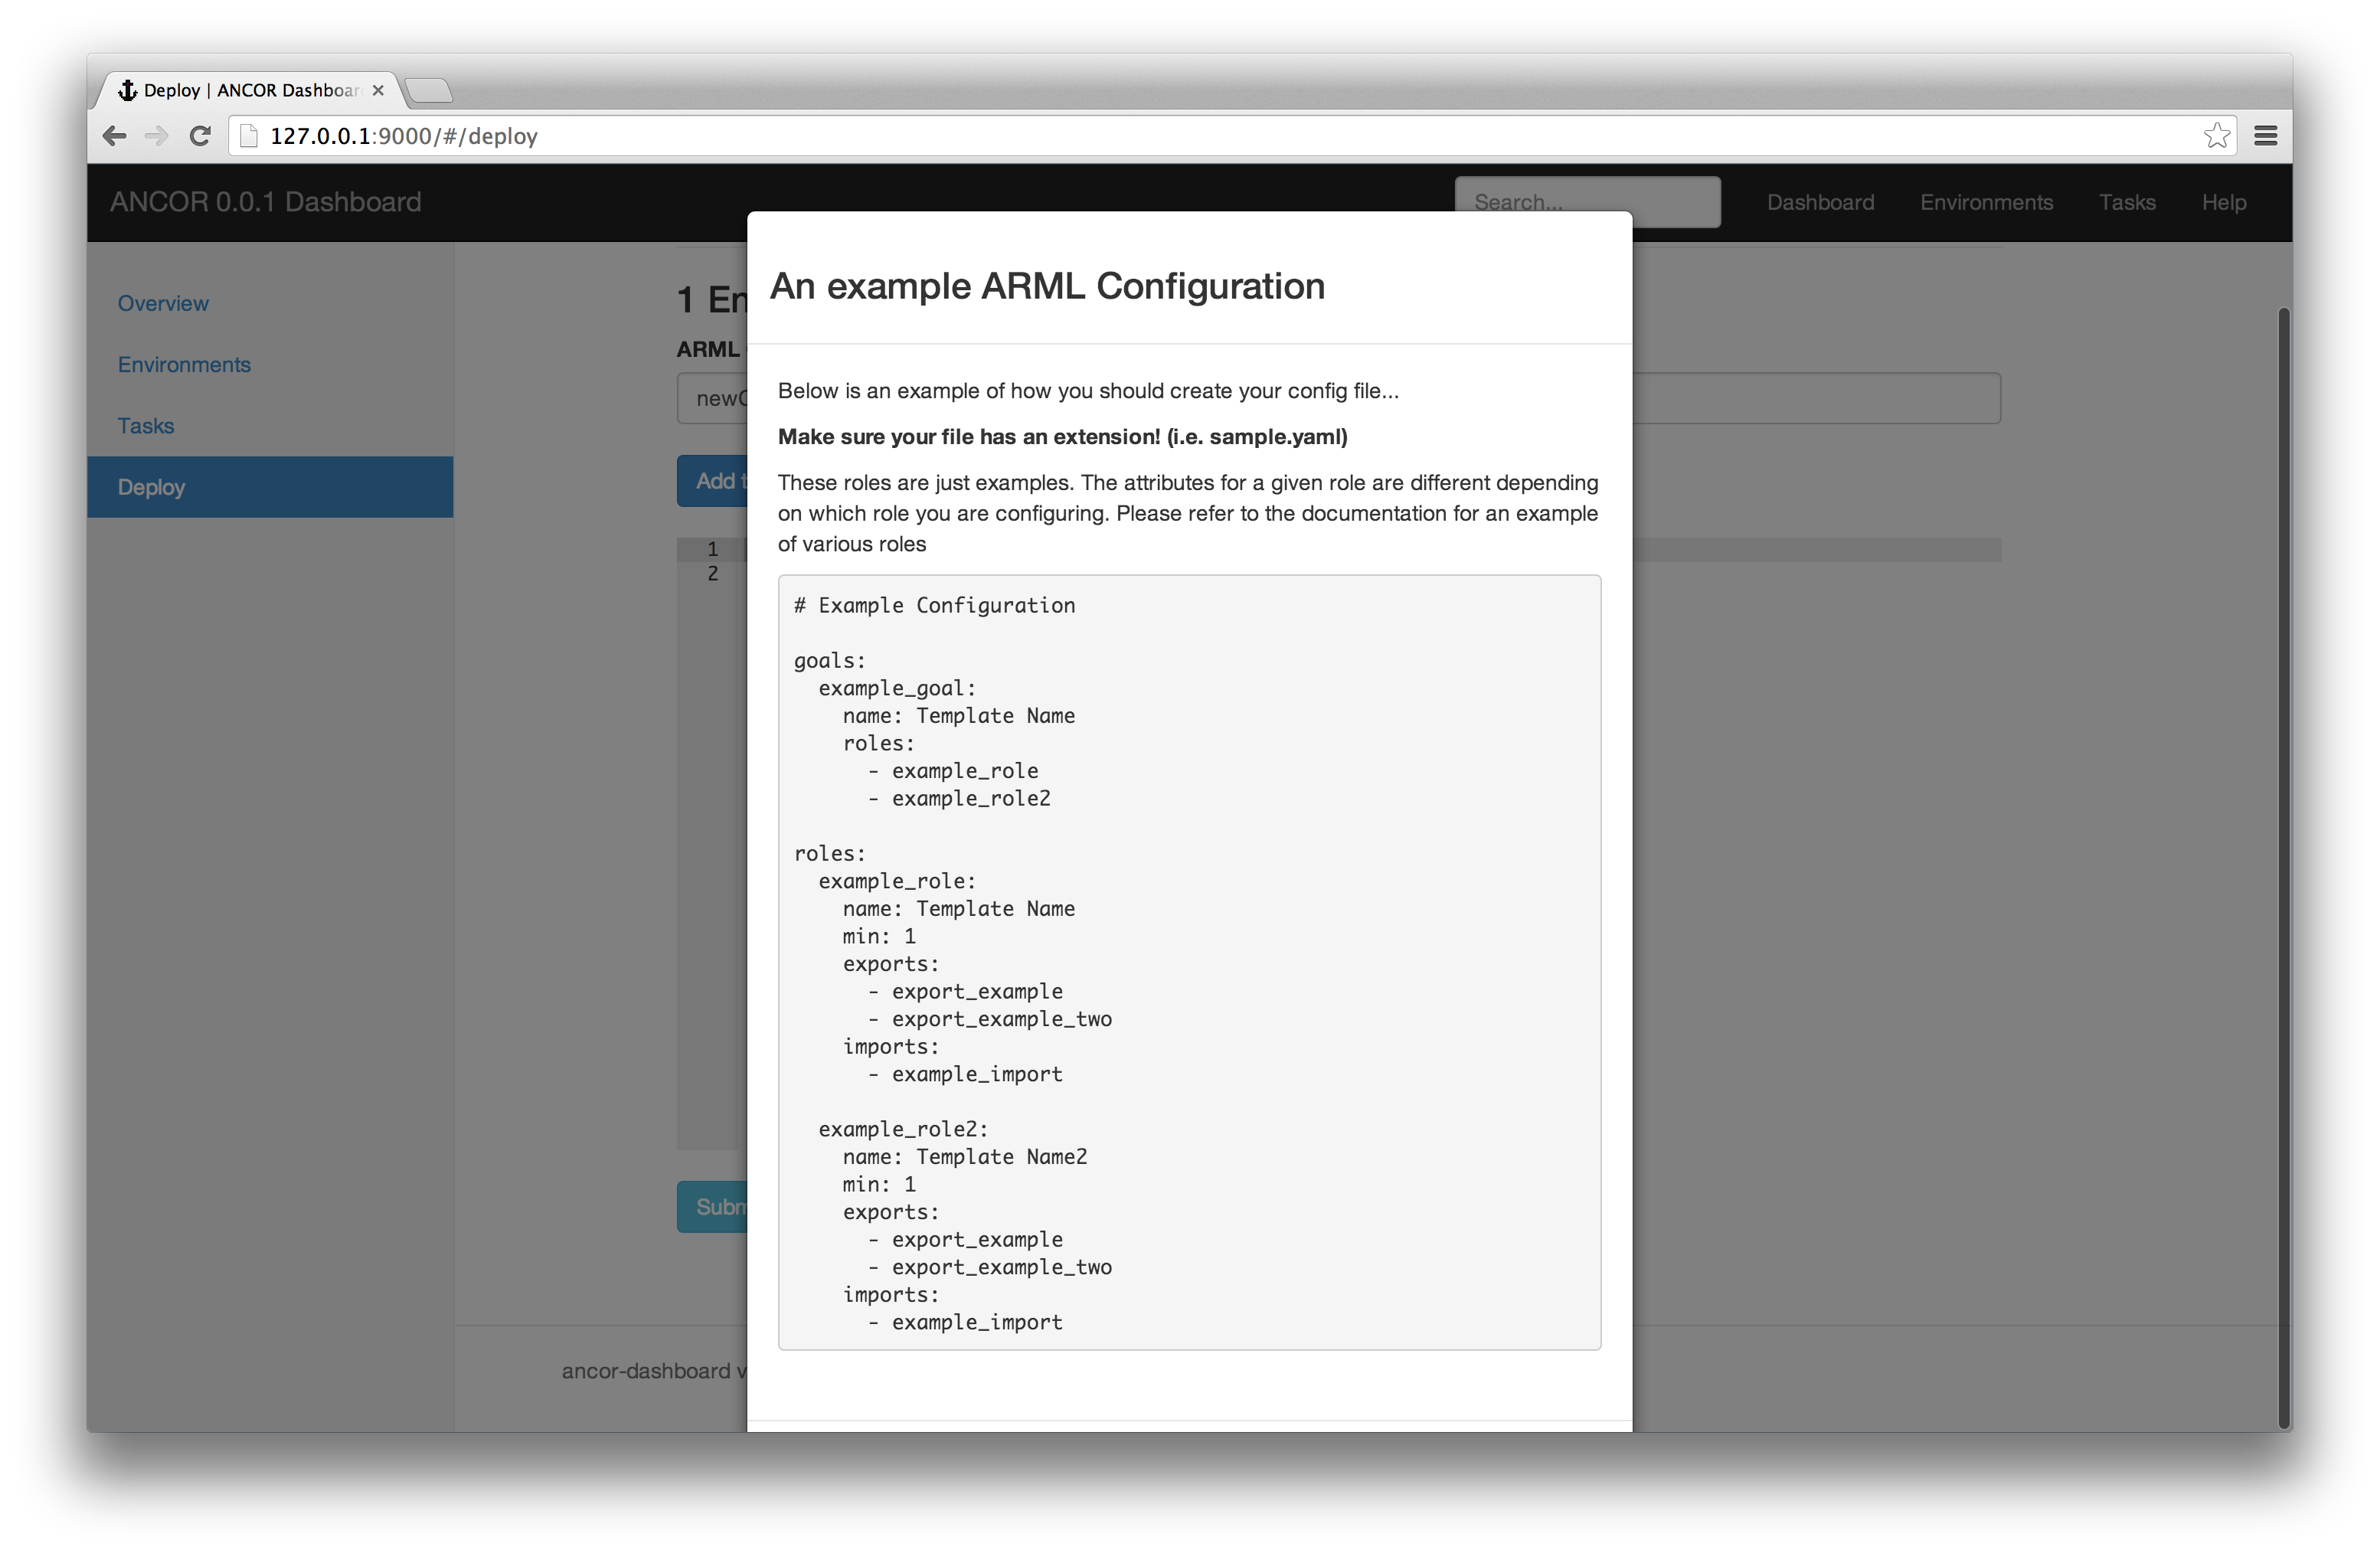
\includegraphics[height=4.0in]{figures/deploy-help.png}

    \caption[Deploy help view.
    ]{The deploy help modal view.}

    \label{deployHelpView}
\end{figure}

\begin{figure}[htb]%t=top, b=bottom, h=here

    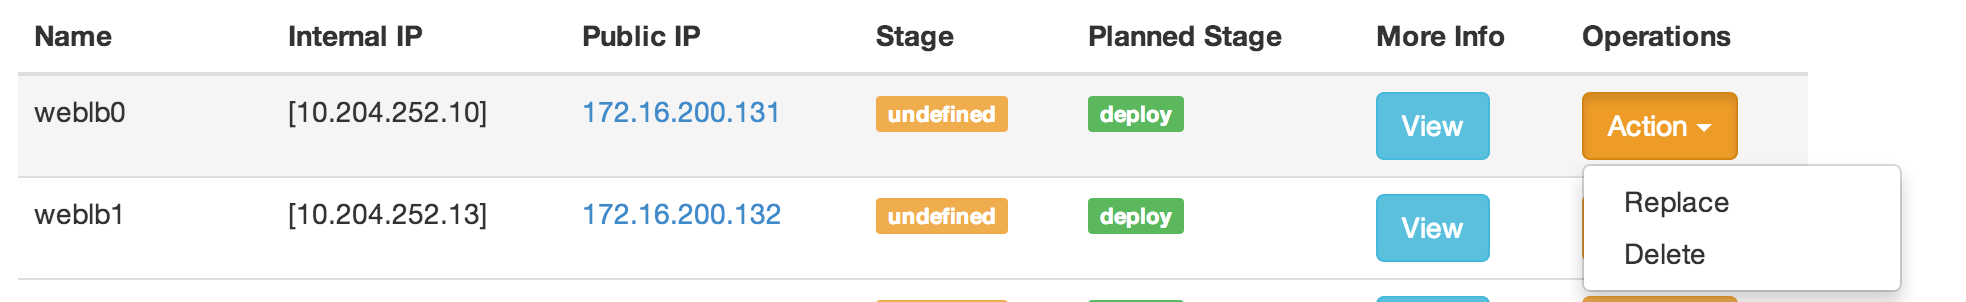
\includegraphics[height=1.0in]{figures/instance-replace-delete.png}

    \caption[Replacing or deleting an instance.
    ]{Replacing or deleting an instance.}

    \label{replaceDeleteInstance}
\end{figure}

\begin{figure}[htb]%t=top, b=bottom, h=here

    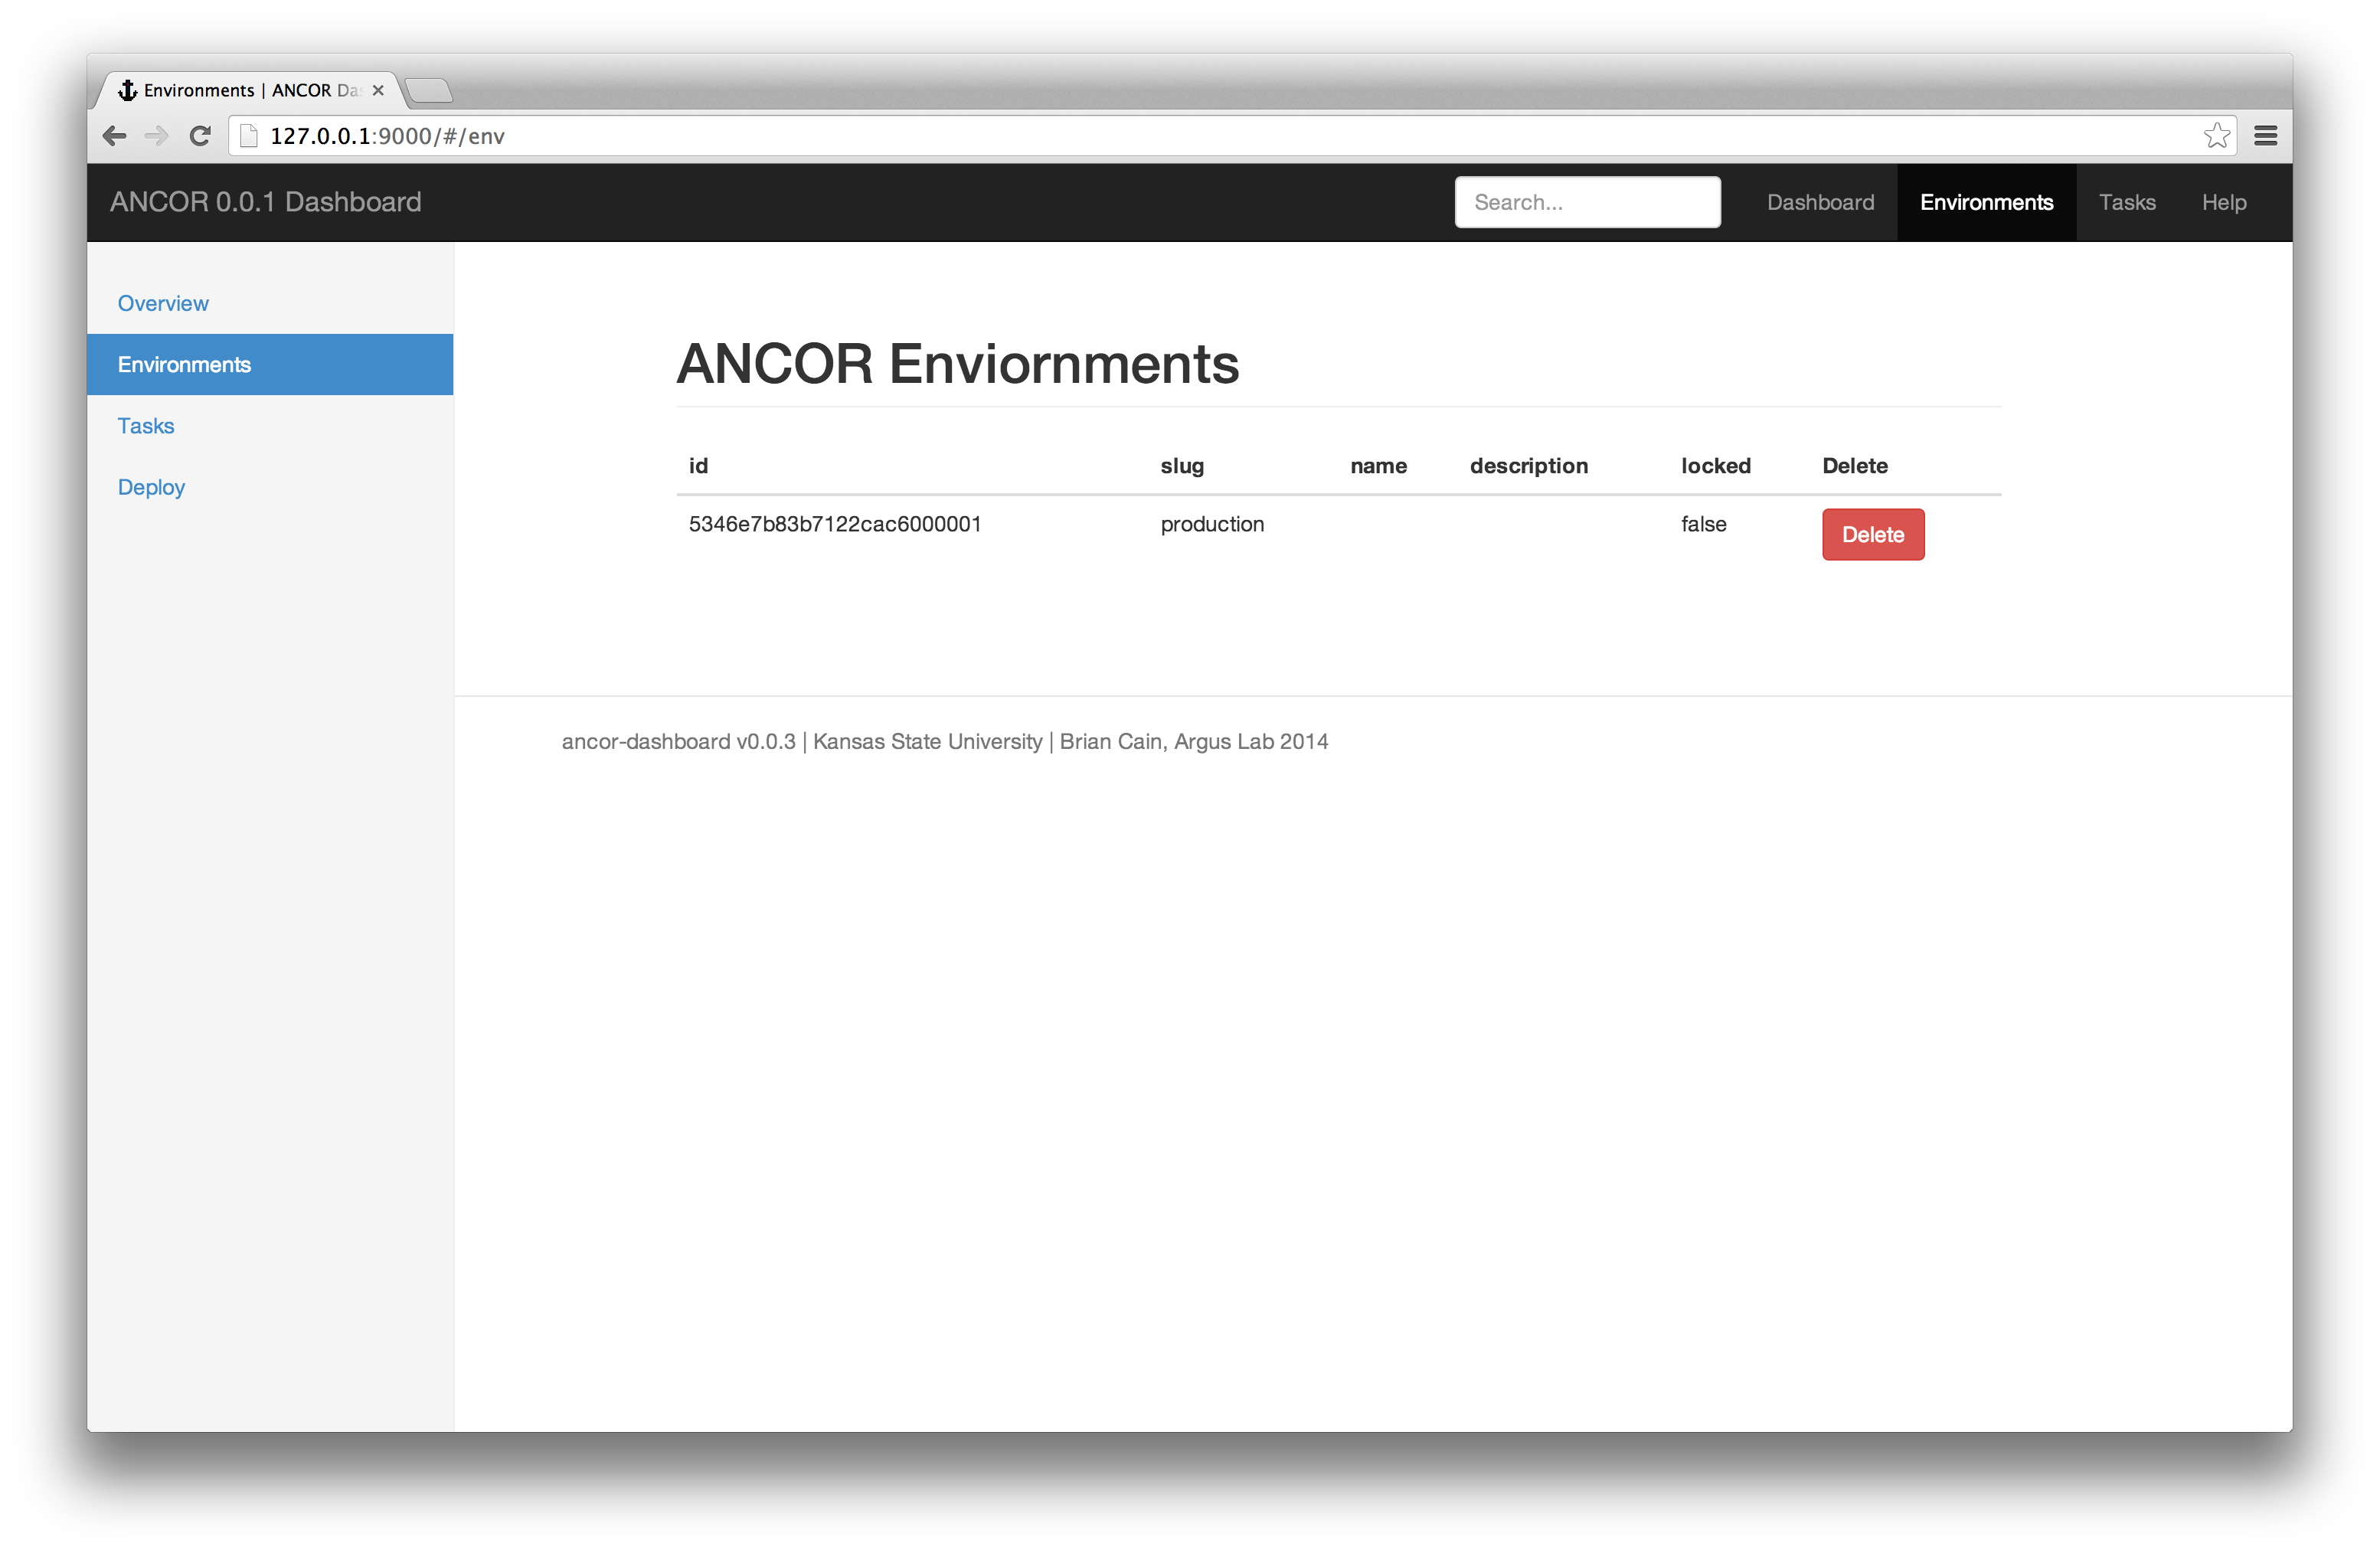
\includegraphics[height=4.0in]{figures/environments.png}

    \caption[Environments view.
    ]{The environments view.}

    \label{envView}
\end{figure}

% +--------------------------------------------------------------------+
% | Enter text for your Appendix page in the space below this box.     |
% |                                                                    |
% +--------------------------------------------------------------------+
